\documentclass{beamer}
\usetheme{Boadilla}

\usepackage{hyperref}
\hypersetup{
  colorlinks = true,
  urlcolor   = blue,
  linkcolor  = blue,
  citecolor  = red
}
\usepackage{graphicx}

% --------------------------------------------------------

\title{Modern data analytics}
\subtitle{COVID-19 analysis}
\author{Sebastiaan Van den Broeck}
\institute{KUL}
\date{\today}

% --------------------------------------------------------

\begin{document}

% Title slide
\begin{frame}
\titlepage
\end{frame}

% Table of content
\begin{frame}
\frametitle{Outline}
\tableofcontents
\end{frame}

% Methodology
\section{Methodology}
\begin{frame}
\frametitle{Methodology}

\begin{figure}
\centering
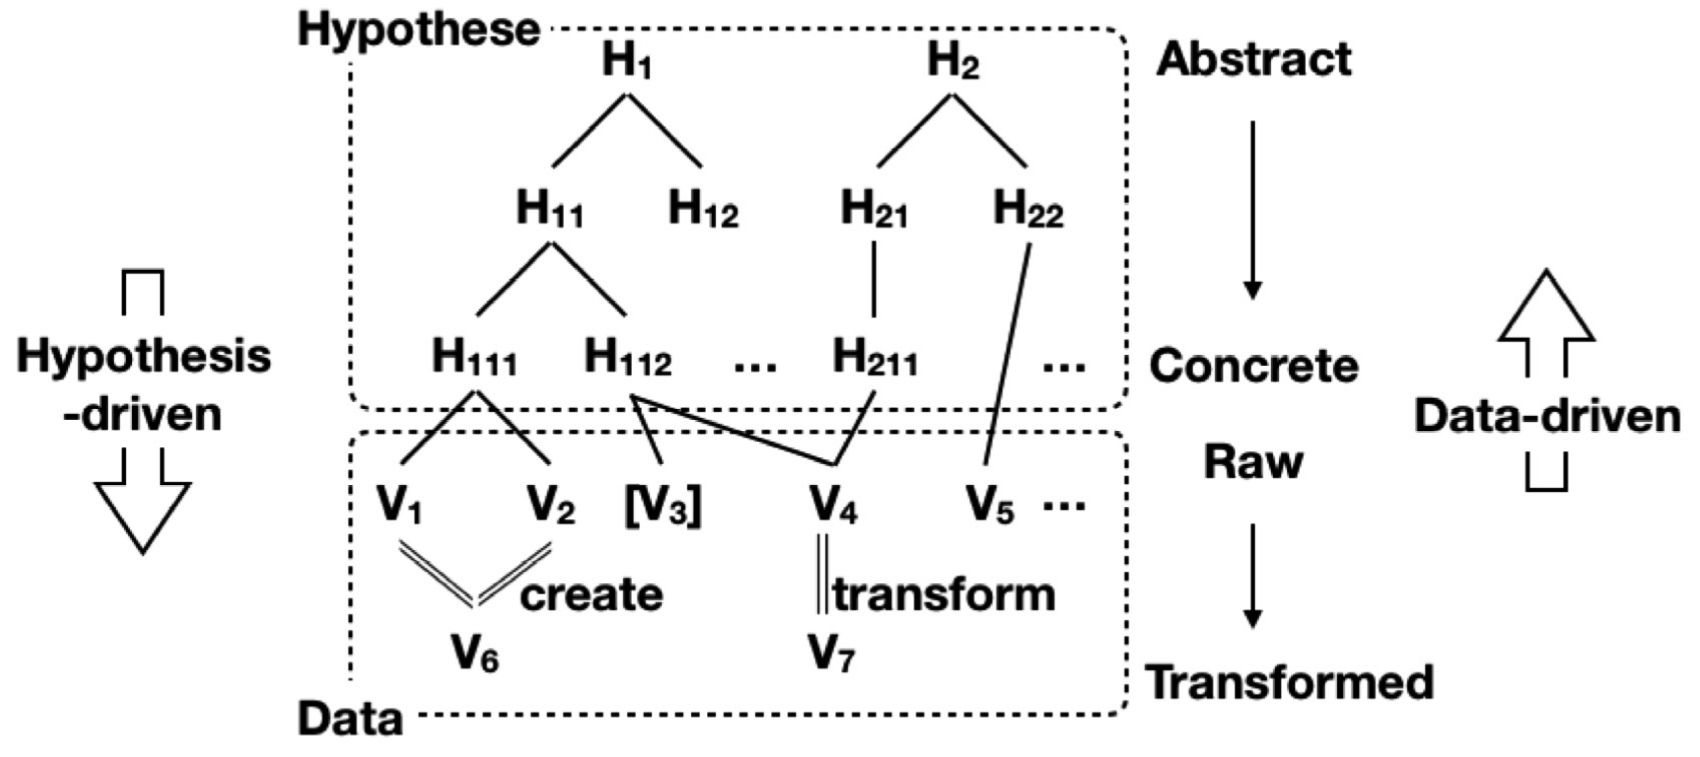
\includegraphics[width=0.8\linewidth]{../visualizations/hypothesis_space_data_space.png}
\end{figure}

\end{frame}

% Data sources
\section{Data sources}
\begin{frame}
\frametitle{Data sources}

\begin{enumerate}
\item \href{https://github.com/nytimes/covid-19-data}{The COVID-19 dataset} \hfill (The New York Times, 2021)
\item \href{https://apps.bea.gov/regional/downloadzip.cfm}{Economical information} \hfill (Bureau of Economic Analysis, 2022)
\item \href{https://zenodo.org/record/6411336\#.YvUG14VBzCl}{The COVID-19 OpenSky dataset} \hfill (Strohmeier et al., 2021)
\item \href{https://github.com/allenai/cord19}{The CORD-19 dataset} \hfill (Lucy et al., 2021)
\end{enumerate}

\end{frame}

% Graph mining
\section{Graph mining}
\begin{frame}
\frametitle{Graph mining}

\begin{figure}
\centering
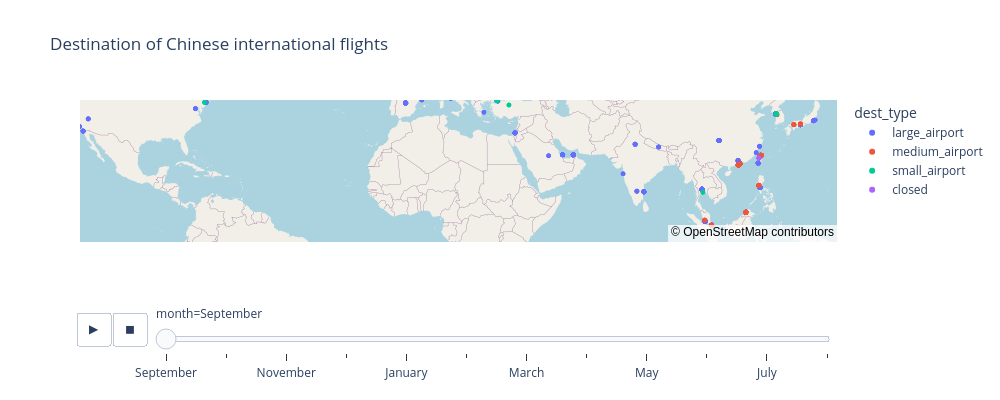
\includegraphics[width=0.8\linewidth]{../visualizations/chinese_flights.png}
\end{figure}

\end{frame}


\begin{frame}
\frametitle{Graph mining}

\begin{itemize}
  \item Degree \hspace{36px} $c_D (i) = \sum_j^N x_{ij}$ \\
    \hspace{72px} where $i, j$ are nodes and $x$ is the adjacency matrix.
  \vfill
  \item Betweenness \hspace{10px} $c_B (i) = \sum_{s, t \in i} \dfrac{\sigma (s, t | i)}{\sigma (s, t)}$ \\
    \hspace{72px} where $i$ is a node, $s$ and $t$ are source and target \\
    \hspace{72px} nodes, $\sigma (s, t)$ is the number of shortest paths \\
    \hspace{72px} between the source and target and $\sigma (s, t | i)$ is the \\
    \hspace{72px} number of shortest paths passing through the node $i$.
  \vfill
  \item Closeness \hspace{25px} $c_C(i) = \left[ \sum_j^N d(i, j) \right]^{-1}$ \\
    \hspace{72px} where $d$ is a distance metric.
\end{itemize}

\vfill

(Brandes, 2008; Opsahl et al., 2010)

\end{frame}


\begin{frame}
\frametitle{Graph mining - the code}

\begin{figure}
\centering
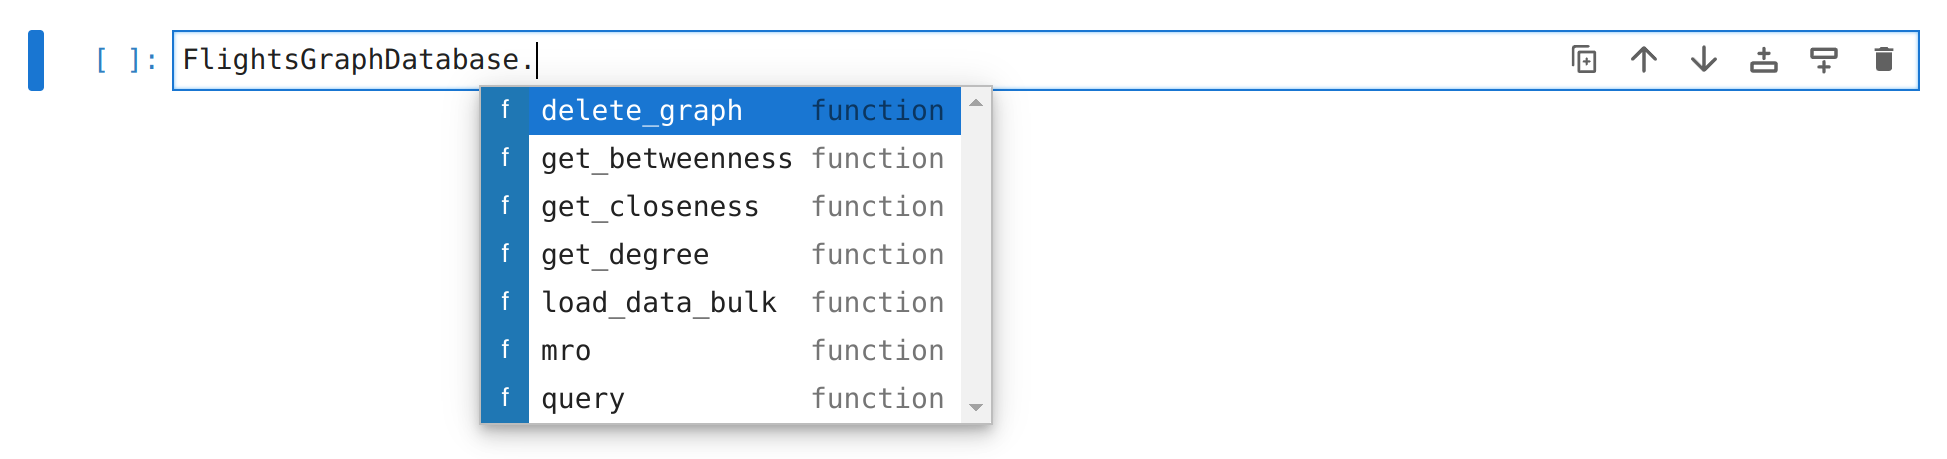
\includegraphics[width=0.8\linewidth]{../visualizations/graph_class_methods.png}
\vfill
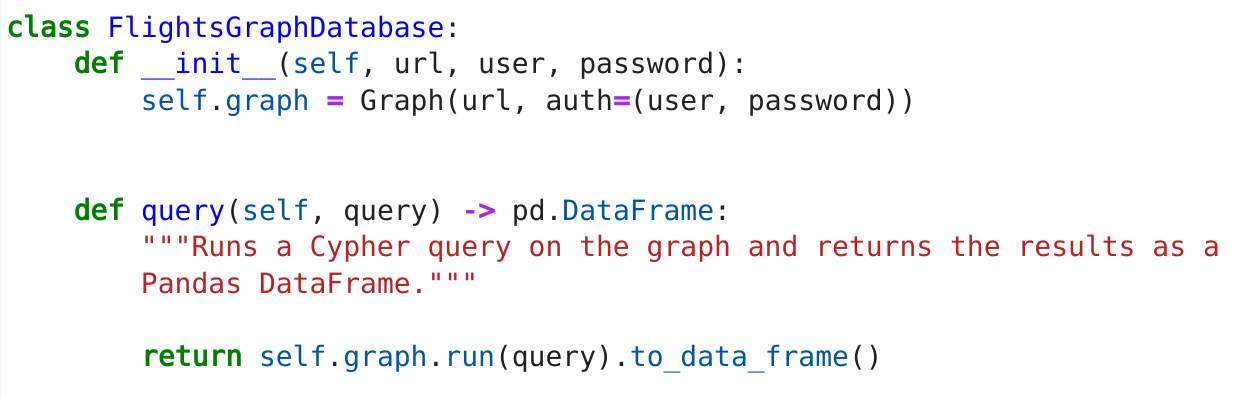
\includegraphics[width=0.8\linewidth]{../visualizations/graph_class_code.png}
\end{figure}

\end{frame}


\begin{frame}
\frametitle{Graph mining - degree centrality}

\begin{figure}
\centering
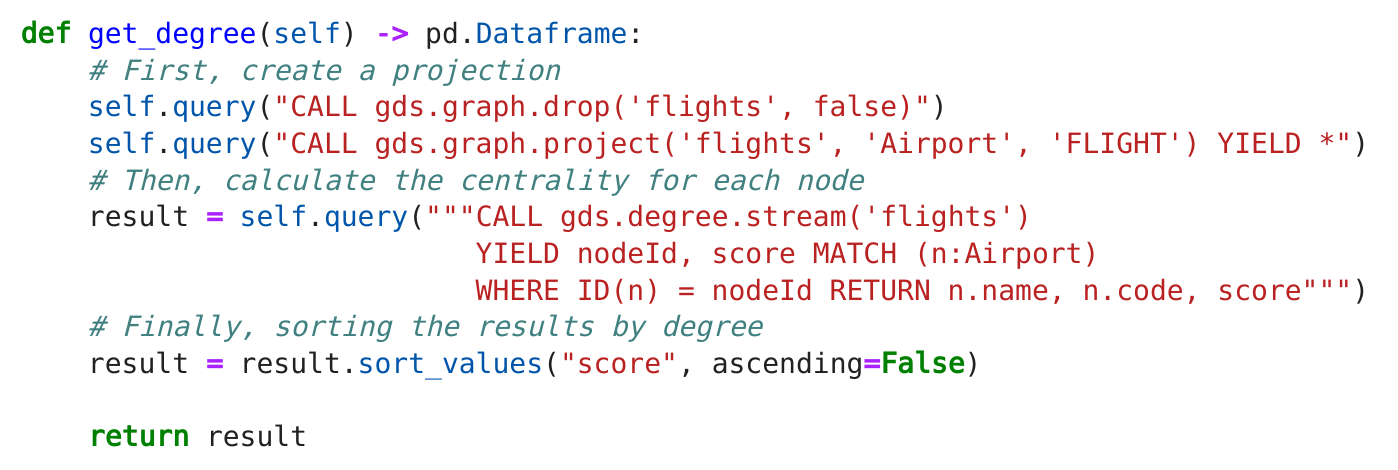
\includegraphics[width=0.6\linewidth]{../visualizations/get_degree_code.png}
\vfill
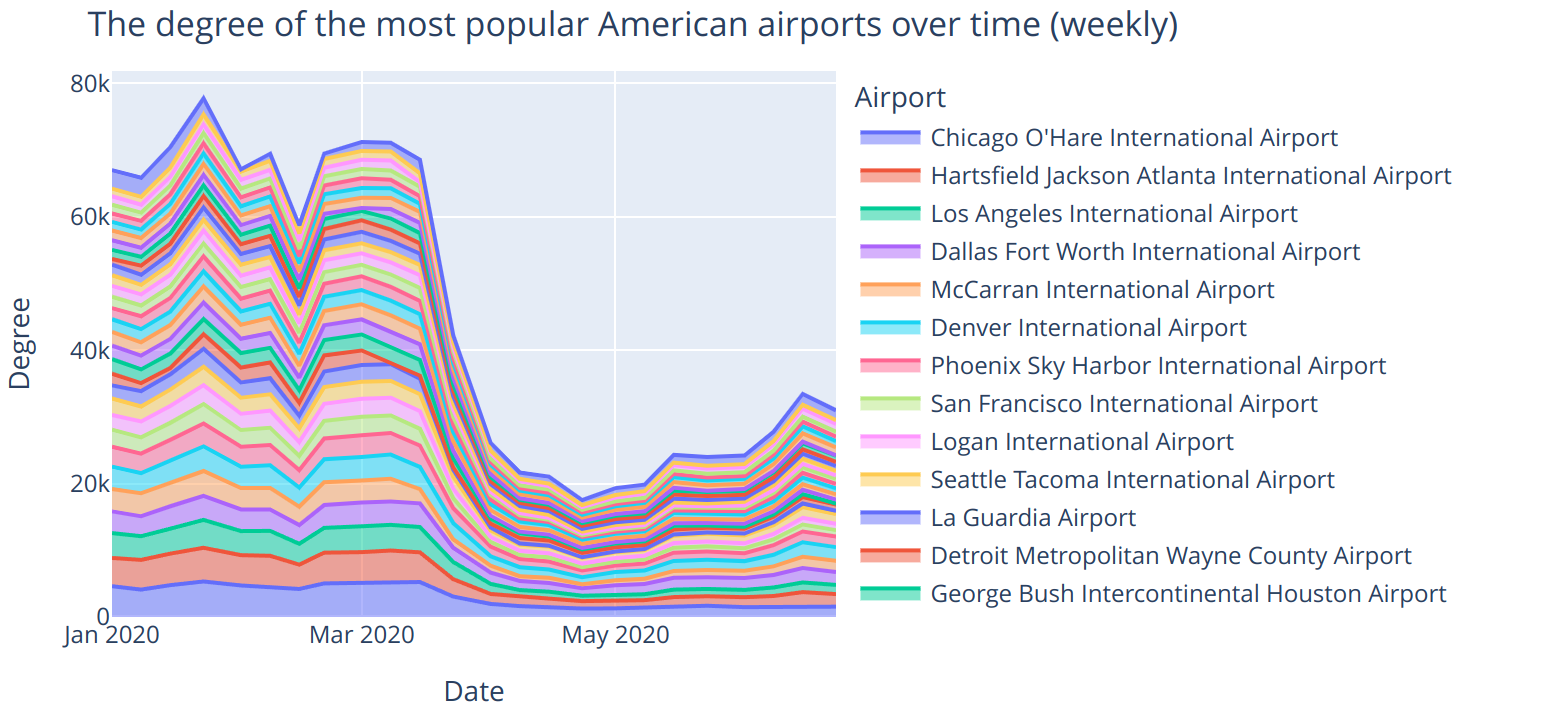
\includegraphics[width=0.6\linewidth]{../visualizations/degree_screenshot.png}
\end{figure}

\end{frame}


\begin{frame}
\frametitle{Graph mining - betweenness centrality}

\begin{figure}
\centering
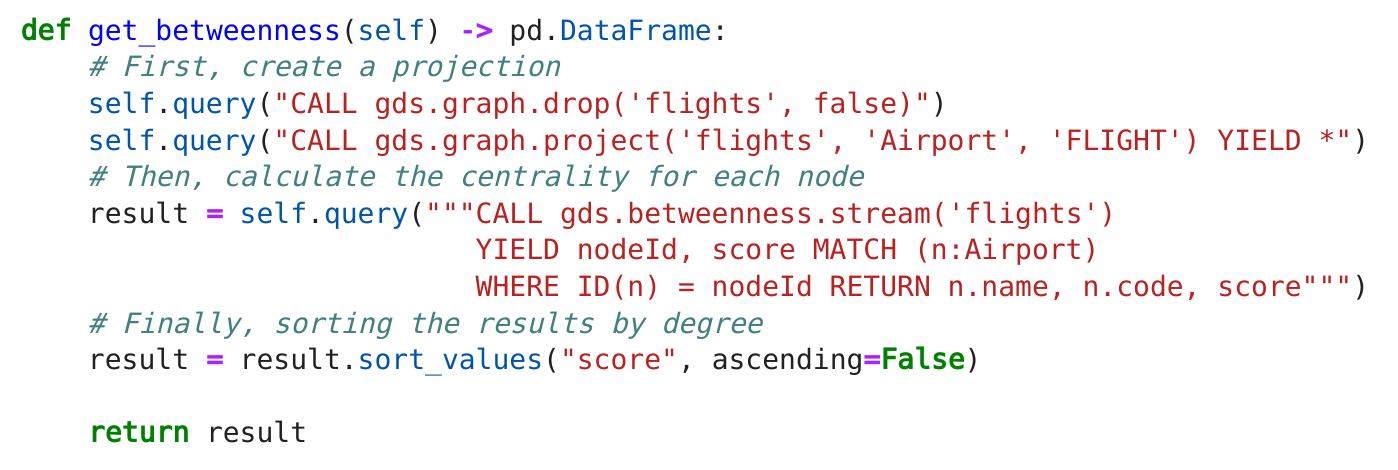
\includegraphics[width=0.6\linewidth]{../visualizations/get_betweenness_code.png}
\vfill
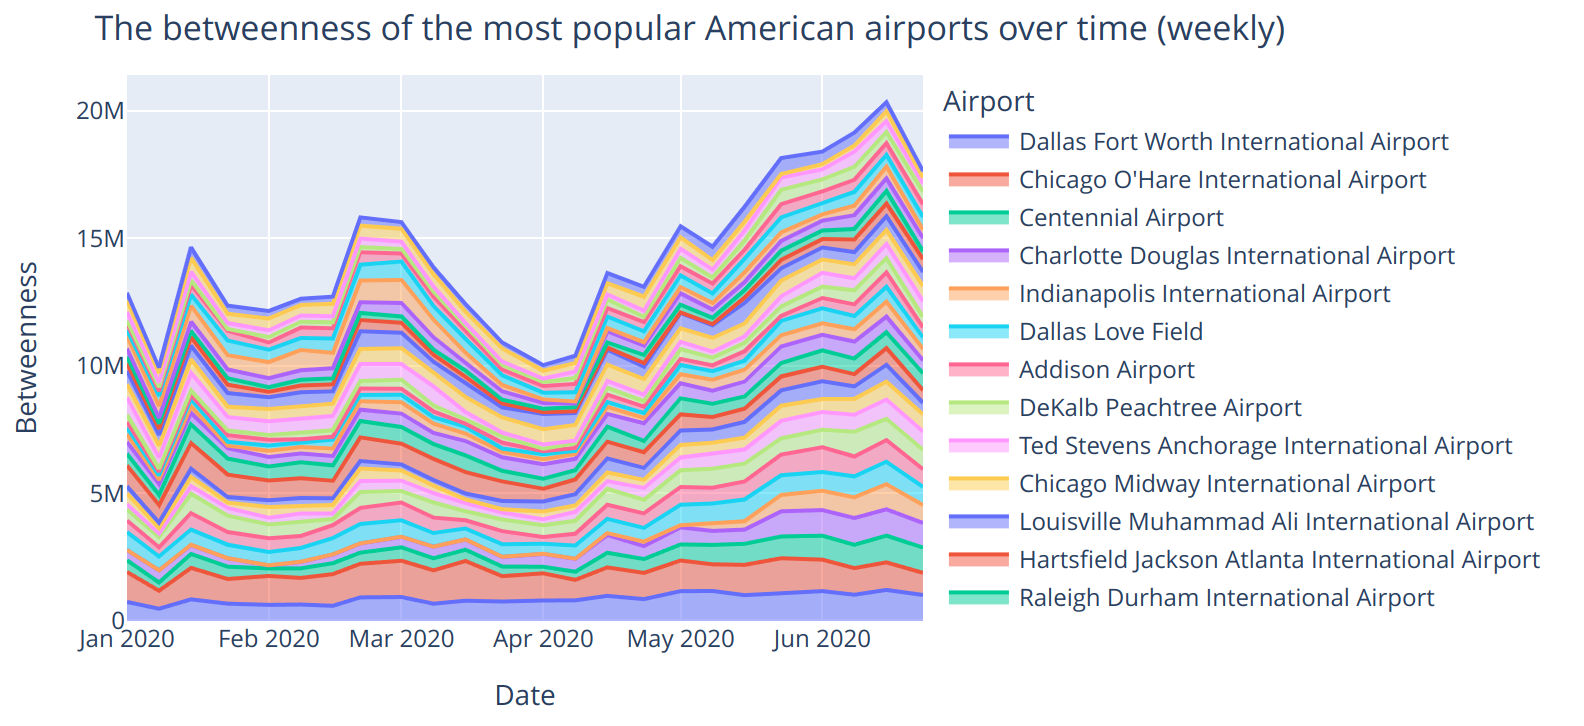
\includegraphics[width=0.6\linewidth]{../visualizations/betweenness_screenshot.png}
\end{figure}

\end{frame}


\begin{frame}
\frametitle{Graph mining - closeness centrality}

\begin{figure}
\centering
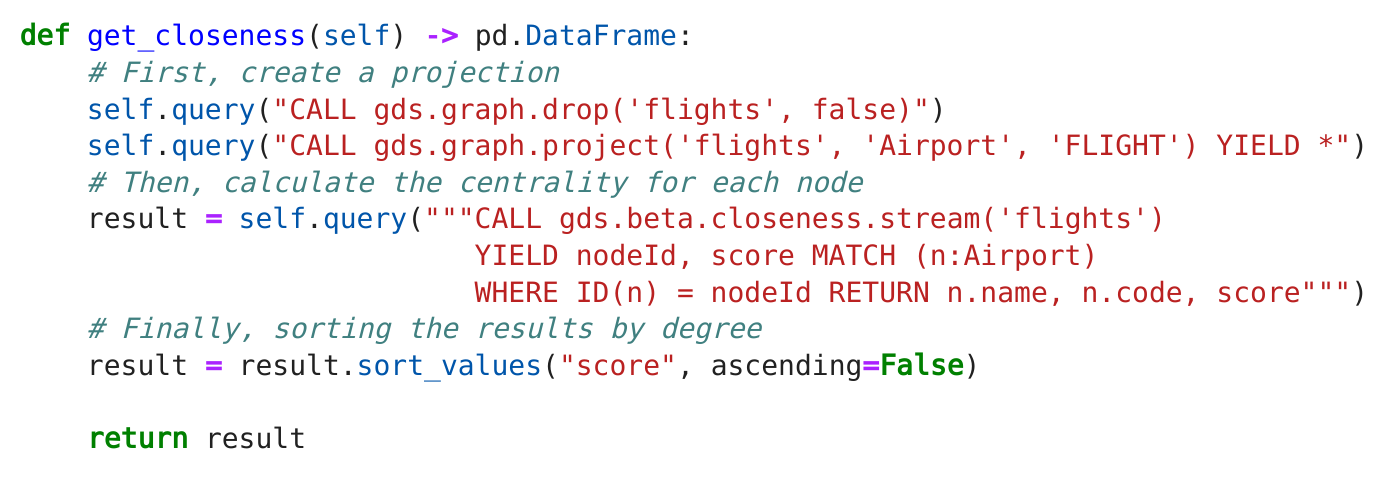
\includegraphics[width=0.6\linewidth]{../visualizations/get_closeness_code.png}
\vfill
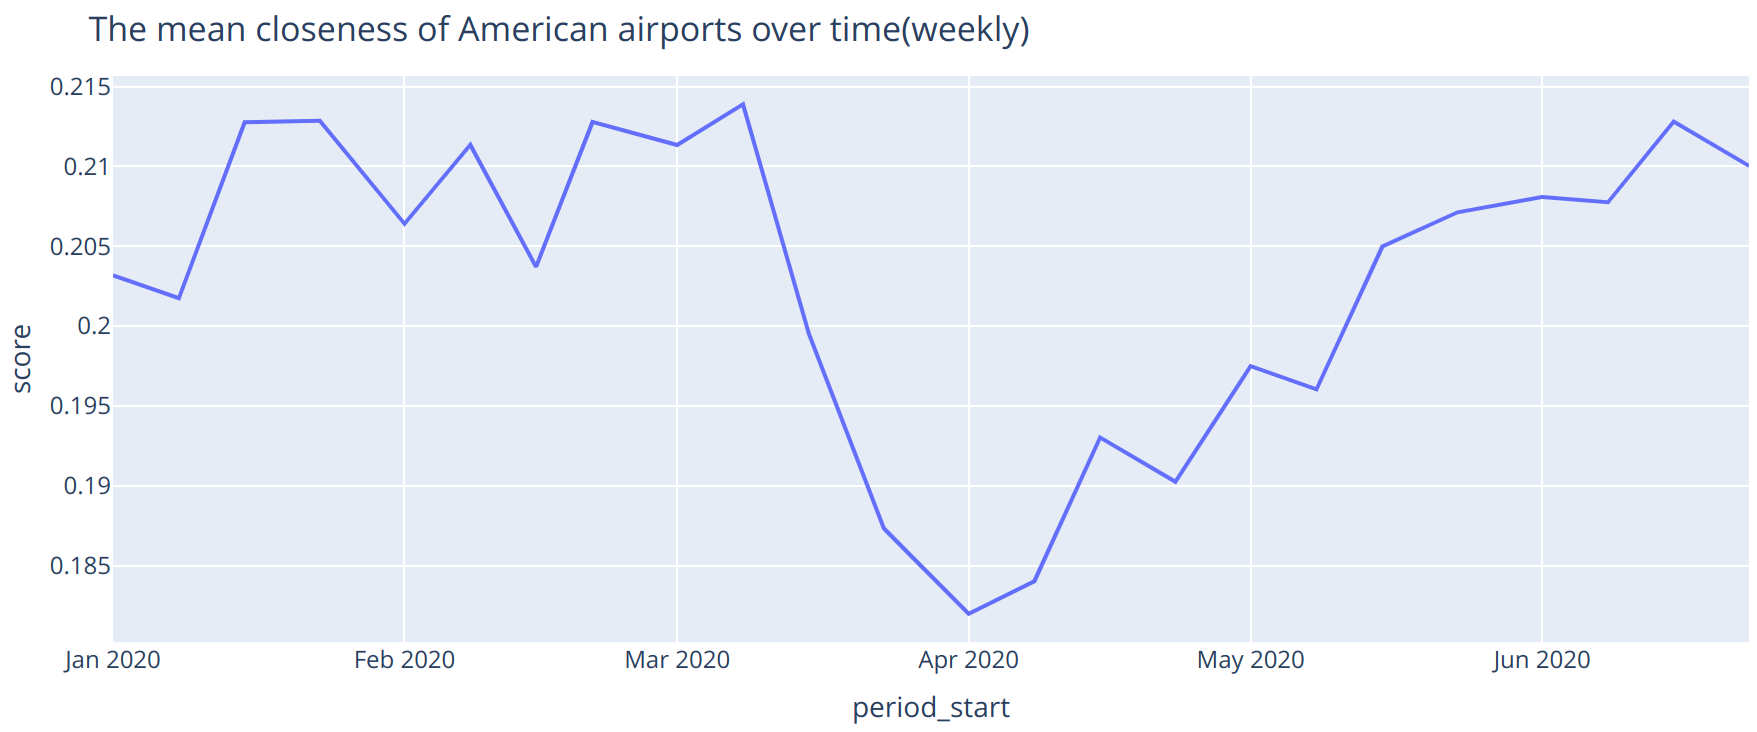
\includegraphics[width=0.6\linewidth]{../visualizations/closeness_screenshot.png}
\end{figure}

\end{frame}

% Text mining
\section{Text mining}
\begin{frame}
\frametitle{Text mining - preprocessing}

\begin{figure}
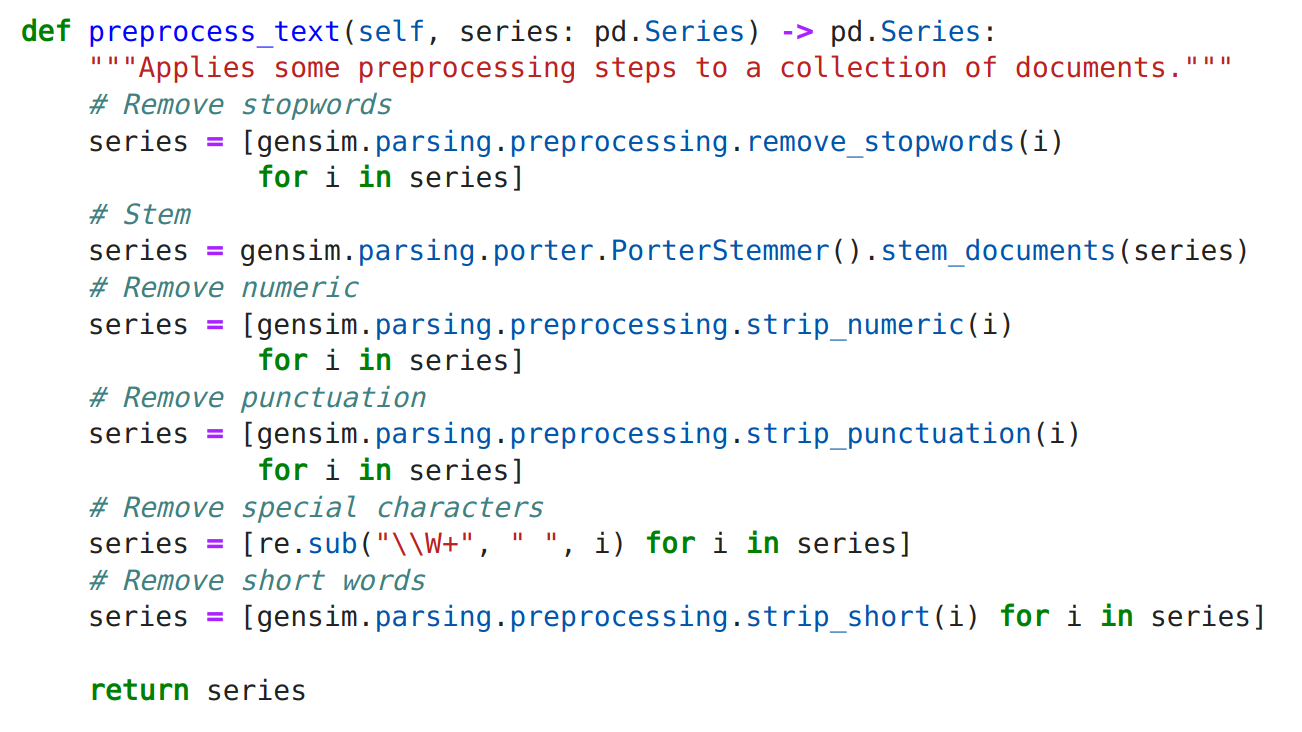
\includegraphics[width=0.6\linewidth]{../visualizations/preprocess_text_code.png}
\end{figure}

\end{frame}


\begin{frame}
\frametitle{Text mining - latent dirichlet allocation}

\begin{figure}
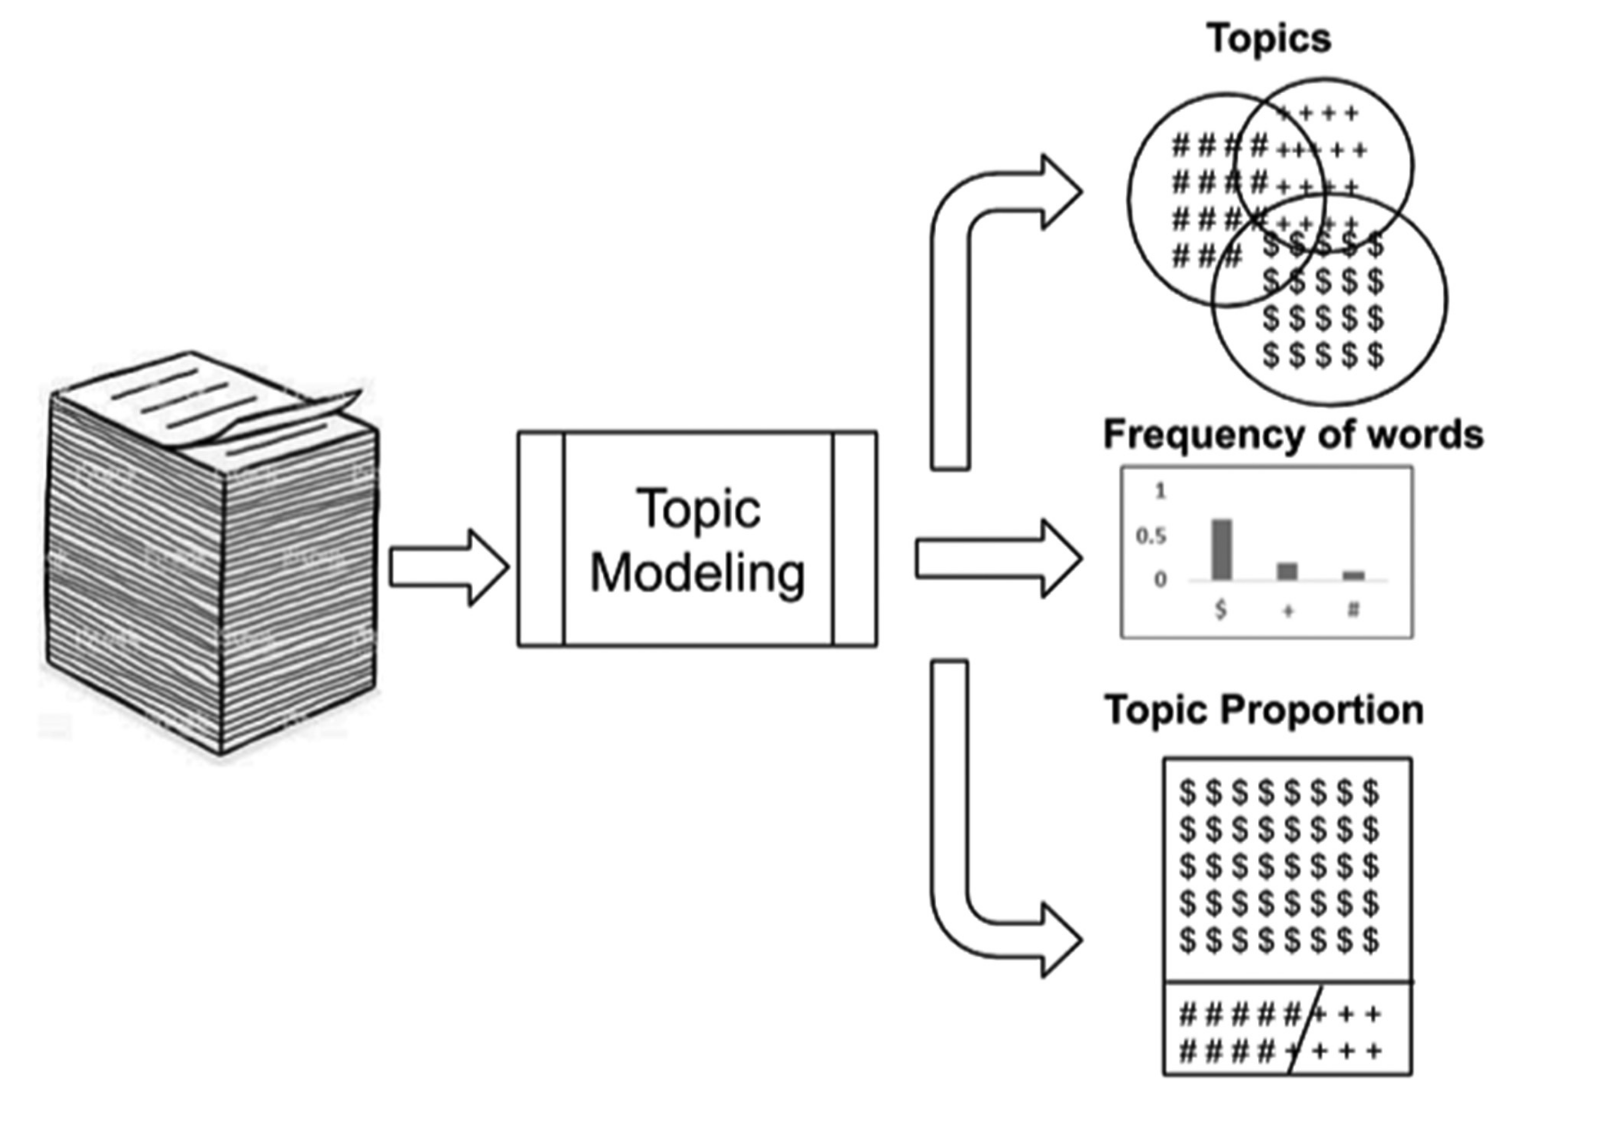
\includegraphics[width=0.6\linewidth]{../visualizations/topic_modelling.png}
\caption{The area of topic modelling is concerned with making inferences from a huge collection of documents in terms of topics, frequency of words and topic proportions. Taken from Chauchan \& Shah (2022)}
\end{figure}

\end{frame}


\begin{frame}
\frametitle{Text mining - before the pandemic}

% Some improvements can still be made regarding preprocessing
% There is a German cluster

% Topic 1 and 5 have to do with the inner workings of a disease and score low on the first PC.
% Topics 2, 3 and 4 score high on the first PC and have more to do with the human and societal impact of a pandemic.

\begin{table}[]
\centering
\scalebox{0.45}{
\begin{tabular}{|l|l|l|l|l|l|l|l|l|l|}
\hline
\textbf{Topic 1} & \textbf{Topic 2} & \textbf{Topic 3} & \textbf{Topic 4} & \textbf{Topic 5} & \textbf{Topic 6} & \textbf{Topic 7} & \textbf{Topic 8} & \textbf{Topic 9} & \textbf{Topic 10} \\ \hline
cell             & health           & patient          & cov              & cell             & infect           & immun            & vaccin           & calv             & der               \\ \hline
protein          & diseas           & respiratori      & detect           & protein          & respiratori      & vaccin           & viru             & protein          & die               \\ \hline
viru             & develop          & studi            & viru             & activ            & viral            & cell             & infect           & viru             & und               \\ \hline
viral            & model            & infect           & sequenc          & lung             & group            & respons          & influenza        & structur         & model             \\ \hline
infect           & public           & associ           & human            & express          & studi            & protein          & studi            & studi            & ein               \\ \hline
activ            & emerg            & children         & respiratori      & induc            & viru             & antigen          & result           & result           & network           \\ \hline
express          & data             & clinic           & virus            & airwai           & associ           & antibodi         & ibv              & effect           & von               \\ \hline
rna              & infecti          & influenza        & pcr              & result           & virus            & specif           & virus            & test             & mit               \\ \hline
virus            & studi            & case             & infect           & increas          & caus             & express          & protect          & differ           & bei               \\ \hline
host             & risk             & hospit           & sars             & mice             & patient          & infect           & effect           & domain           & cell              \\ \hline
\end{tabular}}
\end{table}

\begin{figure}
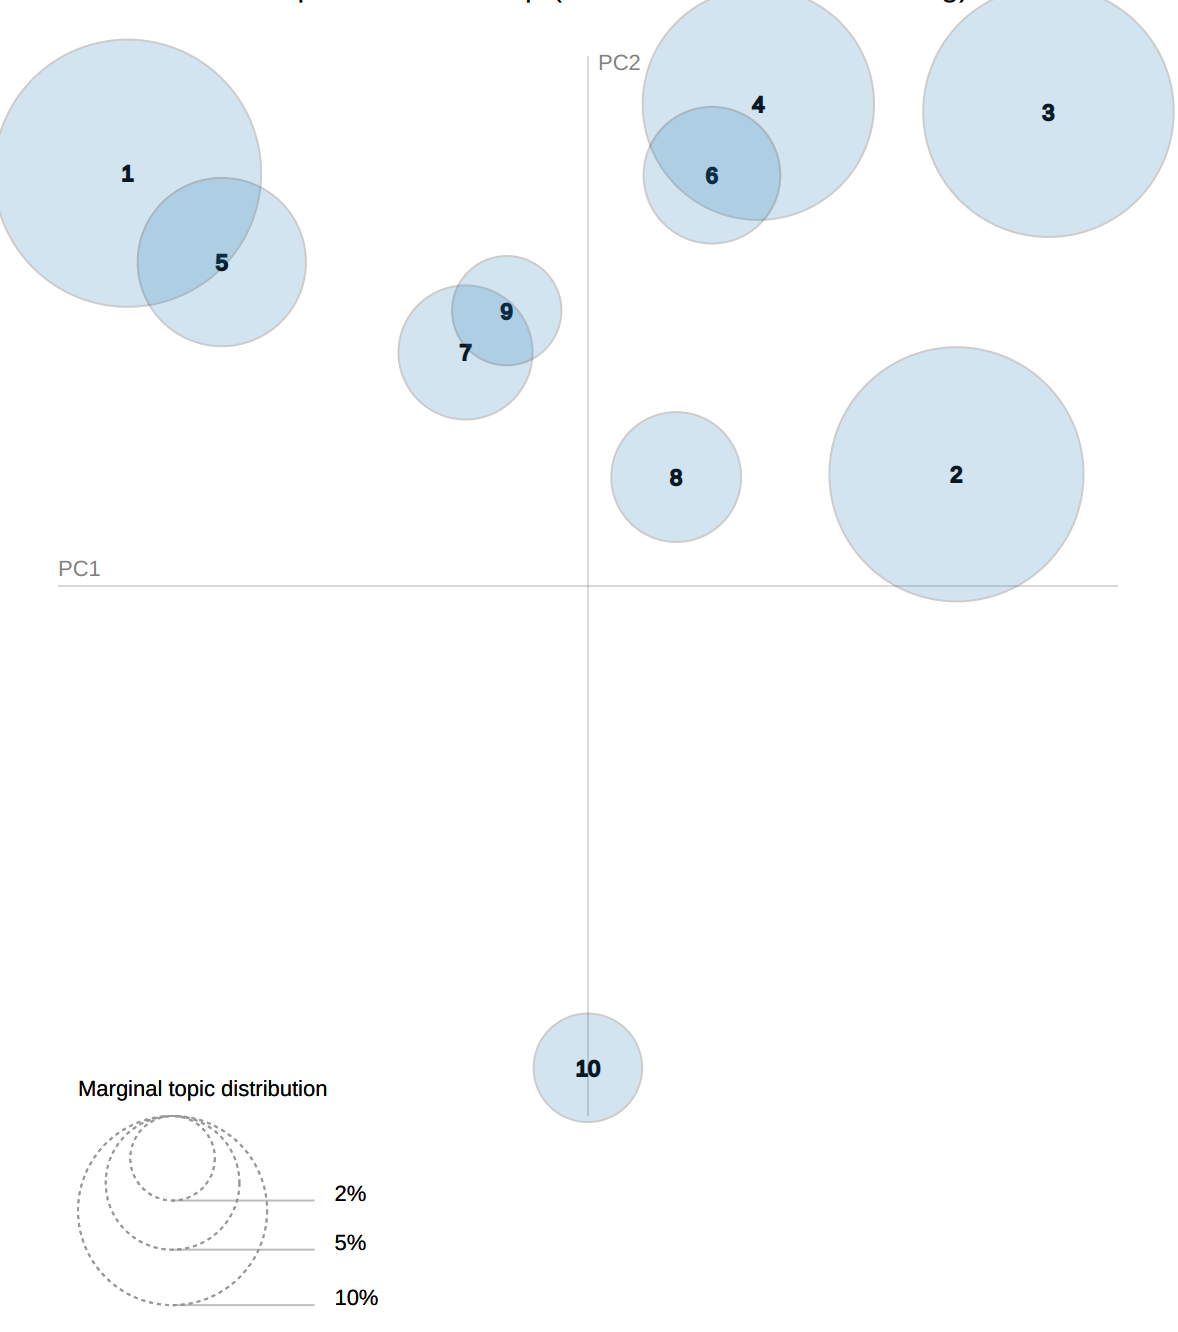
\includegraphics[width=0.4\linewidth]{../visualizations/lda_before_visualization.png}
\end{figure}

\end{frame}


\begin{frame}
\frametitle{Text mining - during pandemic}

% Cluster 9 is new
% German cluster
% There is a cluster dedicated to mental health
% The clusters 1, 3, 4 and 8 score low on the first PC and give an indication of the human and sociatal impact of the pandemic.
% The clusters 6 and 7 score high on the first PC and have more to do with the inner workings of the disease.
% The interpretation of the second PC is a bit less clear to me. Perhaps the treatment of patients is important to obtain a high score here.

\begin{table}[]
\scalebox{0.45}{
\begin{tabular}{|l|l|l|l|l|l|l|l|l|l|}
\hline
\textbf{Topic 1} & \textbf{Topic 2} & \textbf{Topic 3} & \textbf{Topic 4} & \textbf{Topic 5} & \textbf{Topic 6} & \textbf{Topic 7} & \textbf{Topic 8} & \textbf{Topic 9} & \textbf{Topic 10} \\ \hline
health           & patient          & covid            & test             & patient          & cov              & protein          & health           & mask             & der               \\ \hline
covid            & covid            & model            & covid            & cell             & sars             & cov              & studi            & effect           & die               \\ \hline
studi            & hospit           & vaccin           & model            & covid            & covid            & cell             & mental           & covid            & und               \\ \hline
research         & risk             & case             & data             & diseas           & infect           & sars             & depress          & cov              & text              \\ \hline
data             & studi            & studi            & method           & treatment        & patient          & ace              & associ           & sars             & studi             \\ \hline
care             & clinic           & infect           & detect           & immun            & antibodi         & viral            & anxieti          & aerosol          & infect            \\ \hline
pandem           & sever            & number           & perform          & activ            & respiratori      & bind             & women            & patient          & activ             \\ \hline
provid           & associ           & effect           & result           & studi            & coronaviru       & covid            & social           & studi            & gene              \\ \hline
develop          & group            & data             & studi            & clinic           & sever            & viru             & covid            & infect           & effect            \\ \hline
social           & patients         & time             & sampl            & associ           & studi            & drug             & effect           & risk             & model             \\ \hline
\end{tabular}}
\end{table}

\begin{figure}
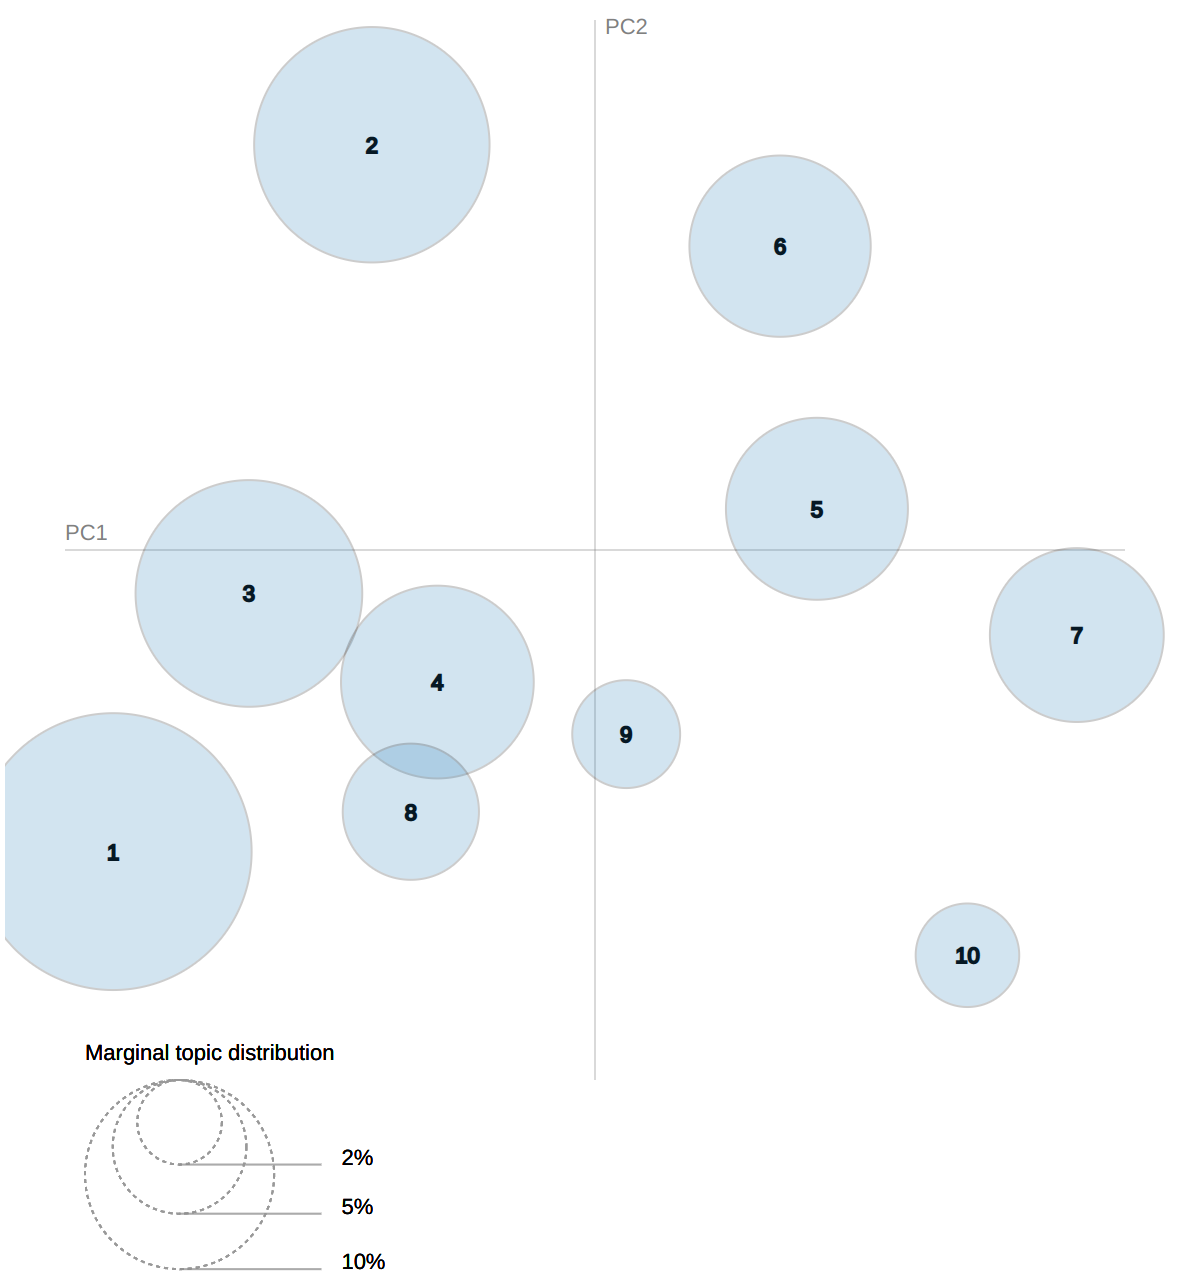
\includegraphics[width=0.4\linewidth]{../visualizations/lda_after_visualization.png}
\end{figure}

\end{frame}


% Sources
\begin{frame}
\frametitle{Sources}

Brandes, U. (2008). On variants of shortest-path betweenness centrality and their generic computation. Social Networks, 30(2), 136–145. \url{https://doi.org/10.1016/j.socnet.2007.11.001} \\

\vspace{5px}

Bureau of Economic Analysis. (2022). Annual GDP per state [Dataset]. \url{https://apps.bea.gov/regional/downloadzip.cfm}

\vspace{5px}

Chauhan, U., \& Shah, A. (2022). Topic Modeling Using Latent Dirichlet allocation: A Survey. ACM Computing Surveys, 54(7), 1–35. https://doi.org/10.1145/3462478

\vspace{5px}

Jelodar, H., Wang, Y., Yuan, C., Feng, X., Jiang, X., Li, Y., \& Zhao, L. (2019). Latent Dirichlet allocation (LDA) and topic modeling: Models, applications, a survey. Multimedia Tools and Applications, 78(11), 15169–15211. \url{https://doi.org/10.1007/s11042-018-6894-4}

\vspace{5px}

Klein, D. J. (2010). Centrality measure in graphs. Journal of Mathematical Chemistry, 47(4), 1209–1223. \url{https://doi.org/10.1007/s10910-009-9635-0}
 
\end{frame}


\begin{frame}
\frametitle{Sources}

Lucy Lu Wang, Kyle Lo, Yoganand Chandrasekhar, Russell Reas, Jiangjiang Yang, Doug Burdick, Darrin Eide, Kathryn Funk, Yannis Katsis, Rodney Michael Kinney, Yunyao Li, Ziyang Liu, William Merrill, Paul Mooney, Dewey A. Murdick, Devvret Rishi, Jerry Sheehan, Zhihong Shen, Brandon Stilson, et al.. 2020. CORD-19: The COVID-19 Open Research Dataset. In Proceedings of the 1st Workshop on NLP for COVID-19 at ACL 2020, Online. Association for Computational Linguistics.

\vspace{5px}

Manríquez, R., Guerrero-Nancuante, C., Martínez, F., \& Taramasco, C. (2021). Spread of Epidemic Disease on Edge-Weighted Graphs from a Database: A Case Study of COVID-19. International Journal of Environmental Research and Public Health, 18(9), 4432. \url{https://doi.org/10.3390/ijerph18094432}

\vspace{5px}

\end{frame}


\begin{frame}
\frametitle{Sources}

Matsumuro, M., \& Miwa, K. (2019). Model for Data Analysis Process and Its Relationship to the Hypothesis-Driven and Data-Driven Research Approaches. In A. Coy, Y. Hayashi, \& M. Chang (Eds.), Intelligent Tutoring Systems (Vol. 11528, pp. 123–132). Springer International Publishing. \url{https://doi.org/10.1007/978-3-030-22244-4_16}

\vspace{5px}

Opsahl, T., Agneessens, F., \& Skvoretz, J. (2010). Node centrality in weighted networks: Generalizing degree and shortest paths. Social Networks, 32(3), 245–251. \url{https://doi.org/10.1016/j.socnet.2010.03.006}

\vspace{5px}

Rehman, S. U., Khan, A. U., \& Fong, S. (2012). Graph mining: A survey of graph mining techniques. Seventh International Conference on Digital Information Management (ICDIM 2012), 88–92. \url{https://doi.org/10.1109/ICDIM.2012.6360146}

\vspace{5px}

Relman, D. A. (2020). To stop the next pandemic, we need to unravel the origins of COVID-19. Proceedings of the National Academy of Sciences, 117(47), 29246–29248. \url{https://doi.org/10.1073/pnas.2021133117}

\vspace{5px}

Sarker, I. H. (2021). Data Science and Analytics: An Overview from Data-Driven Smart Computing, Decision-Making and Applications Perspective. SN Computer Science, 2(5), 377. \url{https://doi.org/10.1007/s42979-021-00765-8}

\end{frame}


\begin{frame}
\frametitle{Sources}


Sievert, C., \& Shirley, K. (2014). LDAvis: A method for visualizing and interpreting topics. Proceedings of the Workshop on Interactive Language Learning, Visualization, and Interfaces, 63–70. \url{https://doi.org/10.3115/v1/W14-3110}

\vspace{5px}

Strohmeier, M., Olive, X., Lübbe, J., Schäfer, M., \& Lenders, V. (2021). Crowdsourced air traffic data from the OpenSky Network 2019–2020. Earth System Science Data, 13(2), 357–366. \url{https://doi.org/10.5194/essd-13-357-2021}

\vspace{5px}

Stroustrup, B. (1988). What is object-oriented programming? IEEE Software, 5(3), 10–20. \url{https://doi.org/10.1109/52.2020}

\vspace{5px}

The New York Times. (2021). Coronavirus (Covid-19) Data in the United States. Retrieved from \url{https://github.com/nytimes/covid-19-data}.

\end{frame}

\end{document}

